\documentclass[a4paper,10pt]{article}

\usepackage{graphicx} 
\usepackage{geometry}
\geometry{
    left=1.5cm,
    right=1.5cm,
    top=1cm,
    bottom=1.5cm
}
\usepackage[english]{babel}

\usepackage{tcolorbox}
\tcbuselibrary{skins}

\addto\captionsenglish{\renewcommand{\figurename}{\textbf{Figure}}}

\usepackage{bootstrapcolors}
\usepackage{capt-of}

\begin{document}

% Task from UVa Online Judge, Problem 929 Number maze
% https://onlinejudge.org/index.php?option=com_onlinejudge&Itemid=8&category=11&page=show_problem&problem=870

\begin{tcolorbox}[enhanced, frame hidden, borderline west = {1.5pt}{0pt}{gray-700},sidebyside,
    sidebyside align=center,lefthand width=10cm,lower separated=false,fontupper=\sffamily]
    \noindent Consider a number maze represented as a two dimensional array of 
    numbers comprehended between $0$ and $9$, as exemplified on the right side. The 
    maze can be traversed following any orthogonal direction (i.e., north, 
    south, east and west). Considering that each cell represents a cost, then 
    finding the minimum cost to travel the maze from one entry point to 
    an exit point may pose a reasonable challenge.
    
    \noindent The task is to find the minimum cost value to go from the top-left 
    corner to the bottom-right corner of a given number maze of size $N \times M$ 
    where $1 \leq N$, $M \leq 999$. Note that the solution for the given example is $24$. \vspace{1mm} \\
    
    \noindent\textbf{Input}\vspace{1mm}
    
    \noindent The input file contains several mazes. The first input line contains a positive integer defining the number 
    of mazes that follow. Each maze is defined by: one line with the number of rows, $N$ ; one line with 
    the number of columns, $M$ ; and $N$ lines, one per each row of the maze, containing the maze numbers 
    separated by spaces.\vspace{1mm} \\
    
    \noindent\textbf{Output}\vspace{1mm}
    
    \noindent For each maze, output one line with the required minimum value.
    
    \tcblower
        \centering
        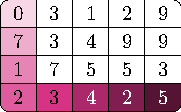
\includegraphics[scale=1.2]{maze_exp.pdf}
            \captionof{figure}{Given Example.}\label{fig:mazeexp}
\end{tcolorbox}

\end{document}